\subsection{High Energy \piz Production}\label{sec:into:xsection.high}
%ere is the citation ~\cite{key1, key2,Rad1996, Diehl}
The production of the \piz meson in photon-proton reactions, for incoming photon beam energies greater than 2.8~GeV, is considered to be a hard exclusive reaction. One approach to study the \piz production, in photon-proton reactions, is use the handbag model. In the handbag approach, the reaction is factorized into two parts. The first part is when one quark from the incoming and one from the outgoing nucleon participate in the hard sub-process, small blob in Fig.~\ref{fig:xsection.handbag}. This hard sub-process is achieved when the incident photon excites a quark, since quarks are bound quantum particles, the excited quark produces a jet of quarks that form the meson and then de-excites back into the nucleon. This is calculable using pQCD. The second part ,the soft part seen as the large blob in Fig.~\ref{fig:xsection.handbag} , consists of all the other quarks that are spectators and can be described in terms of GPDs~\cite{key1, key2,Rad1996, Diehl}. The hard exclusive meson (M) photo-production process factorizes into, $\gamma q \to Mq$, this is depicted in Fig.~\ref{fig:xsection.handbag}. The handbag mechanism is applicable when the Mandelstam variables, $s$, $t$, $u$, are large as compared to a hadronic scale of order 1 GeV . In Ref.~\cite{Huang2000} a model, derived from the handbag approach, has been applied to predict angular dependence of scaled photoproduction cross section of \piz and is illustrated in Fig.~\ref{fig:xsection.handbag.cal}. In the analysis presented, this model will investigated using the data obtained in \abbr{CLAS}.

\begin{figure}[h!]\begin{center}
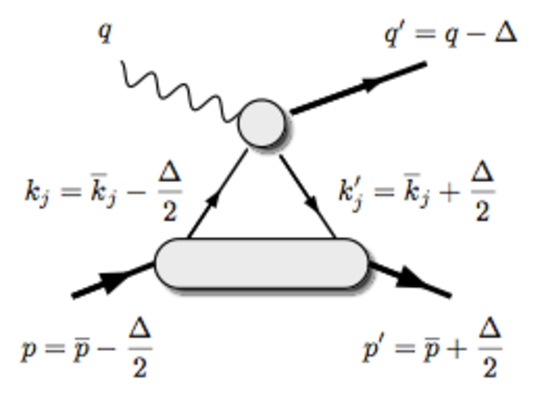
\includegraphics[width= 0.8 \figwidth ,height=\qfigheight]{\grpath/intro/handbag.pdf}
\caption[The handbag-type diagram for photoproduction of mesons]{\label{fig:xsection.handbag}	The handbag-type diagram for photoproduction of mesons. The large blob represents a sum over all spectator configuration. $k_j$ and $k_j^{\prime}$  denote the momenta of the active partons. The small blob stands for meson photoproduction off partons.}
\end{center}\end{figure}

\begin{figure}[h!]\begin{center}
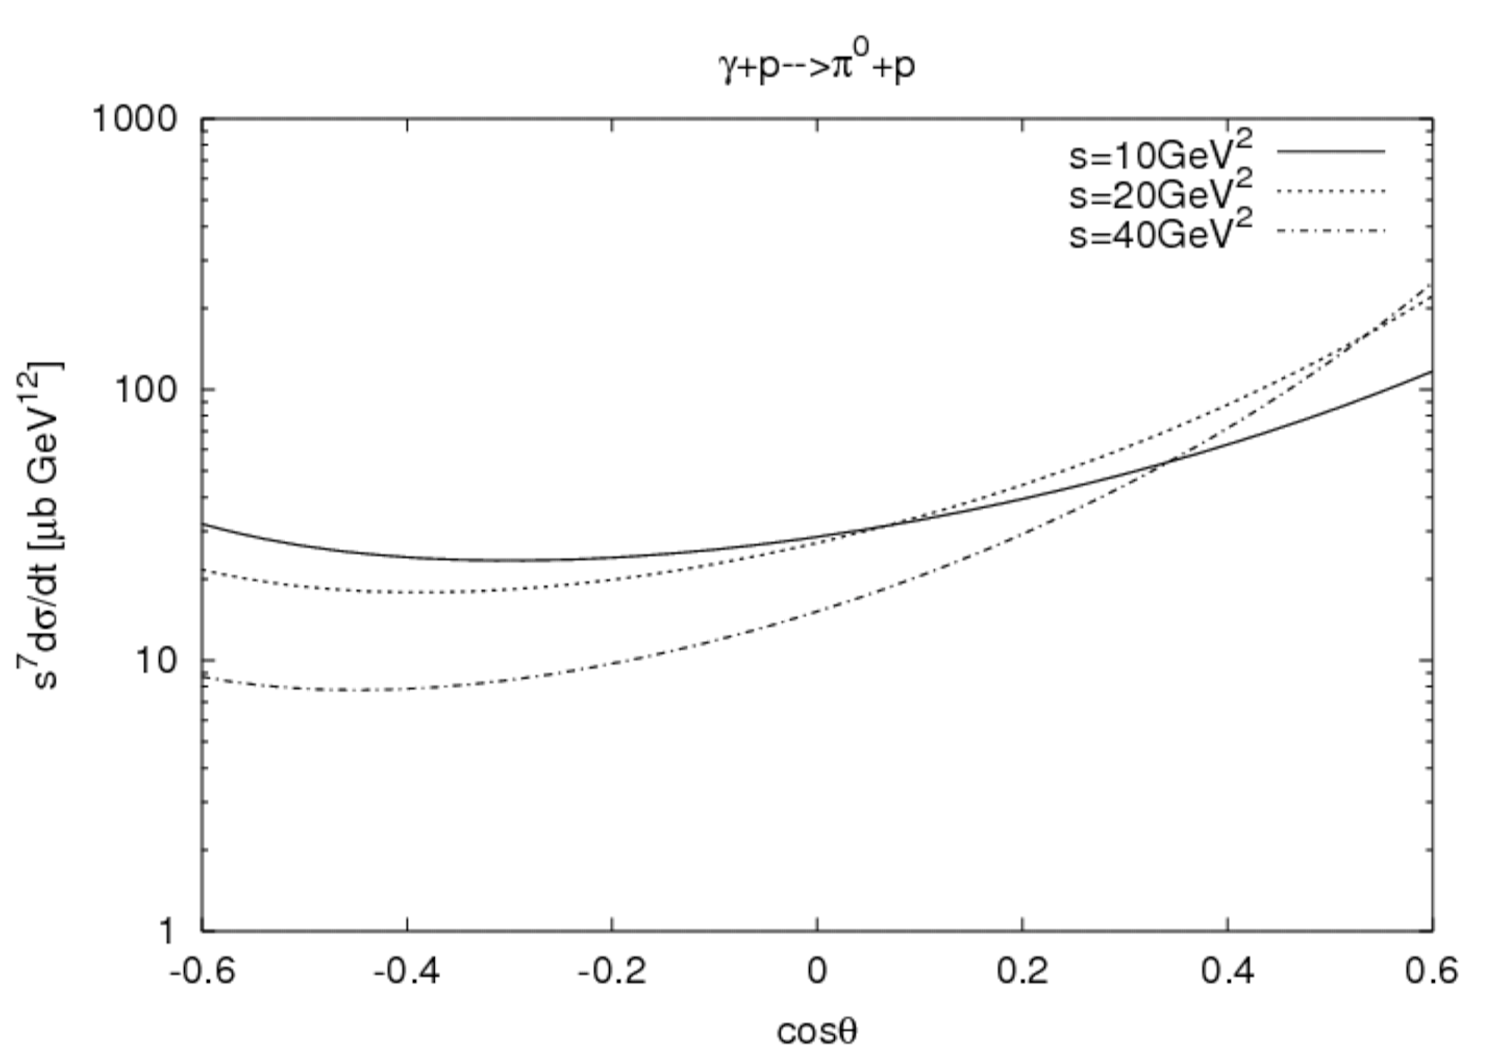
\includegraphics[width= 0.8 \figwidth ,height=\qfigheight]{\grpath/intro/photo-fig7.pdf}
\caption[The soft physics contribution to the cross-section for photoproduction of \piz]{\label{fig:xsection.handbag.cal}The soft physics contribution to the cross-section for photoproduction of \piz scaled by s$^7$ versus $\cos\theta$, where $\theta$ is the scattering angle in the $\gamma p$ c.m. system~\cite{Huang2000}.}
\end{center}\end{figure}
\FloatBarrier


% %